\chapter{Realizacja rozwiązania}
\label{cha:realizacjaRozwiazania}

\par Aby rozwiązać problem przedstawiony w rozdziale \ref{cha:celIMotywacja} postanowiono wykorzystać technologie \dotnet{} i \docker{}. Serwer działa w oparciu o \emph{ASP.NET Core} i \emph{Entity Framework Core}, oraz może zostać uruchomiony zarówno bezpośrednio, jak i w formie kontenera (więcej informacji znajduje się w sekcji \ref{sec:wymaganiaIKonfiguracja}).

\par Komunikacja z aplikacją odbywa się za pomocą protokołu \texttt{\https{}}. \emph{API} przyjmuje i zwraca odpowiedzi w formacie \emph{JSON}\footnote{JavaScript Object Notation}.

\section{Architektura}

\par Odpowiedni podział odpowiedzialności i ustalenie komunikacji między komponentami było jednym z najważniejszych elementów całego projektu. Każdy z komponentów powinien spełniać jasno określone zadania, oraz pewną abstrakcję aby w przypadku późniejszych modyfikacji dało się je łatwo zastąpić. Z tą myślą powstał projekt systemu. Inspiracją dla niego był

\begin{figure}[H]
	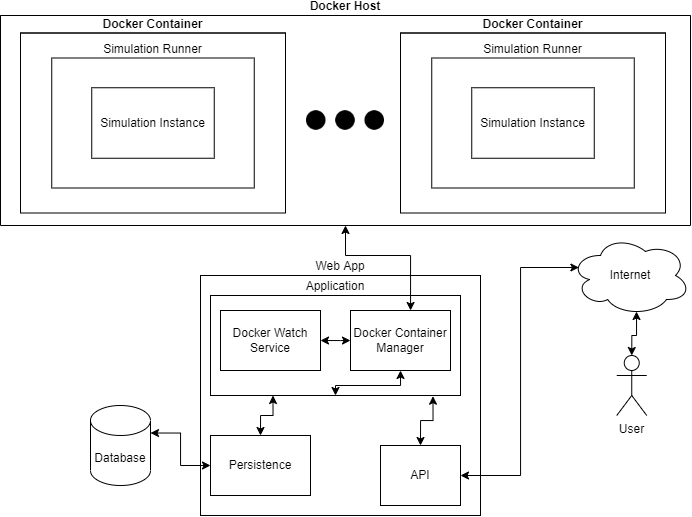
\includegraphics[width=\linewidth]{Component Communication Diagram}
	\caption{Diagram komunikacji między komponentami}
	\label{fig:componentCommunicationDiagram}
\end{figure}

\par Na załączonym powyżej diagramie \ref{fig:componentCommunicationDiagram}, widzimy w jaki sposób komunikują się pomiędzy sobą poszczególne komponenty. Użytkownik wchodzi w interakcję tylko z warstwą \emph{API}, która zajmuje się tylko i wyłącznie obsługą zapytań. Całość logiki biznesowej została oddelegowana do warstwy aplikacji. Ta też warstwa (a konkretnie jej komponent \emph{Docker Container Manger}) jest odpowiedzialna za uruchamianie i zarządzanie kontenerami \emph{\docker{}}a.

\par Za obsługę bazy danych odpowiedzialna jest warstwa \emph{Persistence}. Wszystkie aktywności wymagające przechowania nowych rekordów, aktualizacji lub usunięcia już istniejących są przez nią obsługiwane.

\par \emph{Docker Host} czyli system, na którym jest uruchomiony \emph{\docker{}}. Komunikacja z nim następuje poprzez \emph{Docker Engine API}. Ważnym do zaznaczenia tutaj jest fakt, że może to być albo ten sam \emph{host}, na którym jest uruchomiona nasz aplikacja, ale niekoniecznie musi. Możliwe jest połączanie się z \emph{remote host}em przez internet co prezentuje możliwość na proste poprawienie skalowalności aplikacji w przyszłość. Obecnie jednak założono, że będzie to ten sam \emph{host}, na którym działa aplikacja, co umożliwiło uproszczenie wymiany informacji z kontenerami, która odbywa się poprzez system plików.

\section{Implementacja}

\subsection{Struktura Solucji}

\par W \emph{\dotnet{}} istnieje koncept tak zwanych \emph{solucji}\english{Solutions}. Mają one na celu zgromadzenie w sobie projektów, które razem tworzą rozwiązanie danego zagadnienia. Podejście to pozwala na wyrazisty podział kodu, jak i na wielokrotne jego użycie, zgodne z zasadą \emph{DRY}\footnote{Don't Repeat Yourself}. Odpowiednia zaplanowanie naszego rozwiązania potrafi znacząco przyśpieszyć pracę.

\begin{figure}[H]
	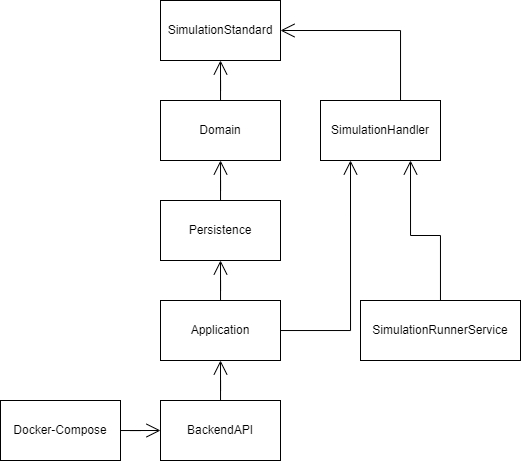
\includegraphics[width=\linewidth]{Solution Structure Diagram}
	\caption{Diagram Struktury Solucji}
	\label{fig:solutionStructureDiagram}
\end{figure}

\par \emph{Docker-Compose} zawiera wszystkie potrzebne informacje do uruchomienia całości rozwiązania, w formie kontenerów \emph{\docker{}}. Umożliwia to uruchomienie aplikacji nie posiadając zainstalowanej platformy \emph{\dotnet{}}, jako iż wszystkie wymagane komponenty zostaną automatycznie pobrane i dodane do odpowiedniego obrazu \emph{\docker{}}.

\par Za punkt wejściowy do naszej aplikacji uznajemy projekt \emph{BackendAPI}. Odpowiada on za uruchomienie i skonfigurowanie wszystkich serwisów. W nim również znajdują się wszystkie kontrolery, logika związana z uwierzytelnianiem użytkownika, jak i pliki konfiguracyjne. \emph{Endpoint}y, które się tutaj znajdują nie posiadają w sobie żadnej logiki biznesowej. Ich zadaniem jest stworzenie odpowiedniego \emph{request}u dla aplikacji, która to dopiero zajmie się jego obsłużeniem.

\par \emph{Application} jest głównym projektem, który spina wszystkie pozostałe. Znajduje się w nim cała logika biznesowa. Odpowiada on za między innymi tworzenie użytkowników i ich autoryzację, zbieranie parametrów i wyników symulacji oraz obsługę pozostałych zapytań, w tym tych związanych z kontenerami (więcej informacji na ten temat znajduje się w sekcjach \ref{sec:dockerContainerManager} i \ref{sec:dockerWatchService}).

\par Odpowiedzialność związana z obsługą symulacji dostarczonych przez użytkowników należy do \emph{SimulationHandler}. Znajdziemy tu interfejs \texttt{ISimulationHandler} i jego implementację. Klasa ta potrafi tworzyć obiekty \emph{SimulationStandard}, w tym przeprowadzać ich serializację i deserializację. Kolejną istotną cechą jest dynamiczne ładowanie i rozładowanie tak zwanych \emph{Assemblies}, jak i sprawdzanie ich poprawność i zgodności z \emph{SimulationStandard}.

\par Projekty \emph{Persistence} i \emph{Domain} odpowiadają za przechowywanie danych. Działają one w oparciu o \emph{Entity Framework Core}. Pierwszy z nich odpowiada za rozszerzenie tak zwanego \emph{DbContext}\footnote{Specjalna klasa pochodząca z Entity Framework Core definiująca pewien kontekst danych.}, w którym znajdują się deklaracje kolekcji, które będą mapowane do poszczególnych tabel w bazie danych. Znajdują się tutaj również migracje, wspomagające ciągły rozwój aplikacji, poprzez zapewnianie mechanizmu do prostego aktualizowania przechowywanych danych w wypadku zmiany ich struktury. Projekt \emph{Domain} reprezentuje z kolej poszczególne byty na których operuje nasza aplikacja. Są one bezpośrednio mapowane do odpowiednich rekordów. Warstwa ta została zaprojektowana przy pomocy tak zwanego podejścia \emph{Code First}. Oznacza to, że odpowiednie struktury w bazie danych zostały automatycznie wygenerowane na podstawie zdefiniowanych klas.

\par Zadaniem \emph{SimulationRunnerService}u jest uruchomienie wyznaczonej symulacji z odpowiednimi parametrami oraz późniejsze zapisanie wyników. Serwis ten funkcjonuje jako osobny \emph{\docker Image}, który jest uruchamiany jako kontener przez \texttt{IDockerContainerManager}. Całość komunikacji pomiędzy poszczególną instancją i resztą systemu odbywa się przez system plików (więcej informacji na ten temat znajduje się w sekcji \ref{sec:dockerContainerManager}).

\par \emph{SimulationStandard} definiuje strukturę jaką powinna spełniać symulacja przygotowana przez użytkownika, jak i jej obsługiwane typy danych parametrów oraz rezultatów. Temu tematowi poświęcona jest sekcja \ref{sec:simulationStandard}.

\subsection{Zastosowane Wzorce Projektowe}

% TODO Add to bibliography sources for Design Patterns
\par Wzorce projektowe pozwalają programistą w szybszy sposób zaznajomić się z aplikacją, poprzez dodanie kolejnej warstwy aplikacji, jak i rozwiązać problemy, które już kiedyś zostały rozwiązane. Należy jednak pamiętać, że trzeba umiejętnie z nich korzystać i rozważyć zarówno korzyści, jak i potencjalne mankamenty, które mogą z nich wyniknąć. Mając to na uwadze, zdecydowano się użyć następujących \emph{Design Patterns}.

\begin{itemize}
	\item Model View Controller TODO % TODO
	\item Dependency Injection TODO % TODO
	\item Data Transfer Object TODO % TODO
	\item Singleton TODO % TODO
\end{itemize}

\subsection{Simulation Standard}
\label{sec:simulationStandard}

\subsection{Docker Container Manager}
\label{sec:dockerContainerManager}

\subsection{Docker Watch Service}
\label{sec:dockerWatchService}

\subsection{Schemat Bazy Danych}

\section{Wymagania i Konfiguracja}
\label{sec:wymaganiaIKonfiguracja}

\section{Endpoints}

\section{Obsługa błędów}

